\documentclass{article}
\usepackage{fancyhdr} % Required for custom headers
\usepackage{lastpage} % Required to determine the last page for the footer
\usepackage{extramarks} % Required for headers and footers
\usepackage{graphicx} % Required to insert images
%\usepackage{lipsum} % Used for inserting dummy 'Lorem ipsum' text into the template
\usepackage{amsmath}
%\usepackage{amsfont}
%\usepackage{amssymb}

\usepackage{multicol}
% Margins
\topmargin=-0.5in
\evensidemargin=0in
\oddsidemargin=-0.5in
\textwidth=7.5in
\textheight=9.0in
\headsep=0.25in 


\pagestyle{fancy}

\rhead{M. Adam} % Top right header
\lhead{Asparagus Torta}
\chead{ }
%\title{}

\begin{document}
%
%PRELIMINARIES:
%
%
%Begin by preheating the oven to 350 $^o$F
%
%\bigskip
%
%\bigskip

\begin{multicols}{2}
Ingredients:
\begin{itemize}
\item 1/2 bunch of fresh asparagus
\item 1/2 onion, chopped
\item 1 garlic clove
\item 4 eggs
\item 1/4 cup gluten-free Panko breadcrumbs
\item 1/4 cup grated Parmesan cheese
\item 1/8th tsp salt Pepper, to taste
\item Butter greasing the pie dish 2 tbsp olive oil sautéing
\end{itemize}



\columnbreak

Directions:
\begin{enumerate}
\item Preheat oven to 325-350°F.

\item Sautee chopped onions and garlic in olive oil over medium heat until glassy.

\item Add chopped asparagus and sauté until tender, remove from heat.

\item Whisk eggs together while asparagus is cooling.

\item Add sautéed vegetables, panko crumbs, grated parmesan, salt, and pepper to egg mixture and combine with whisk

\item Generously grease a glass or ceramic pie dish with butter and pour the mixture into the dish.

\item Bake for about 20 minutes or until firm and beginning to turn golden brown.

\item Cool and serve.
\end{enumerate}
\end{multicols}



\begin{center}
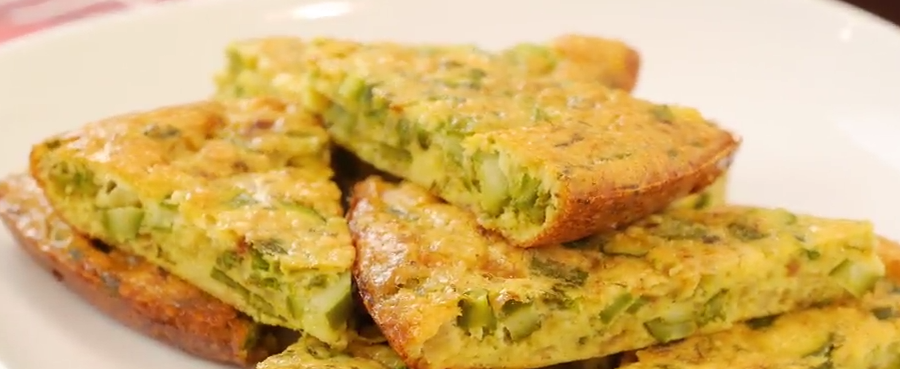
\includegraphics[scale=0.4]{AsparagusTorta.png}
\end{center}


\end{document} 











